\documentclass[11pt,a4paper]{article}
\usepackage{iftex}
\ifPDFTeX
  \usepackage[T1]{fontenc}
  \usepackage{lmodern}
  \usepackage[utf8]{inputenc}
\else
  \usepackage{fontspec}        % XeTeX/LuaTeX (ex. tectonic) : UTF-8 natif, guillemets « » corrects
\fi
\usepackage[french]{babel}
\usepackage[a4paper,margin=2.2cm]{geometry}
\usepackage{amsmath,amssymb}
\usepackage{booktabs}
\usepackage{longtable}
\usepackage{array}
\usepackage{enumitem}
\usepackage{graphicx}
\usepackage{xcolor}
\usepackage{tcolorbox}
\usepackage{hyperref}
\hypersetup{colorlinks=true,linkcolor=blue!50!black,urlcolor=blue!50!black,citecolor=blue!50!black}
\usepackage{titlesec}
\titlespacing{\section}{0pt}{1.5em}{0.5em}
\titlespacing{\subsection}{0pt}{1.0em}{0.3em}
\setlength{\parindent}{0pt}
\setlength{\parskip}{0.45em}
\newcommand{\code}[1]{\texttt{\small #1}}
\newcommand{\E}{\mathbb{E}}
\newtcolorbox{keybox}[1]{colback=blue!4,colframe=blue!40!black,title=\textbf{#1}}
\newtcolorbox{defbox}[1]{colback=gray!6,colframe=gray!50,boxrule=0.4pt,left=5pt,right=5pt,top=3pt,bottom=3pt,title=\textbf{#1}}

\title{\textbf{Congress Trading Signal}\\[4pt]
\large Copier les trades déclarés du Congrès américain bat-il le marché ?\\
\large \emph{Méthodes, mathématiques et résultats --- rapport de recherche}}
\author{Alice Lemaire \quad---\quad Semaines 3--4 : stratégie \& backtest
\quad(\code{06\_Recherche\_Strategie\_2014\_2026.ipynb})}
\date{\today}

\begin{document}
\maketitle

\begin{defbox}{Comment lire ce rapport}
Ce document est \textbf{autonome} : toutes les méthodes (avec leurs formules) et tous les résultats y sont
expliqués sans qu'il soit nécessaire d'ouvrir le code. Il est \textbf{calqué sur le notebook}
\code{06\_Recherche\_Strategie\_2014\_2026.ipynb} --- mêmes sections \S1--\S8, mêmes exemples calculés à la
main, mêmes chiffres (chaque valeur citée ici est la sortie d'une cellule ; correspondance en
annexe~\ref{app:trace}). Le notebook est \textbf{auto-suffisant} : il construit lui-même son cache de prix
au premier lancement, puis s'exécute entièrement hors-ligne.
\end{defbox}

\begin{keybox}{Résumé exécutif}
\textbf{Question.} Les transactions déclarées par les élus américains (STOCK Act) contiennent-elles un
signal qu'un investisseur extérieur peut copier --- sachant qu'il ne les voit qu'à leur \emph{publication},
0--45~jours après le trade ?\\[2pt]
\textbf{Réponse : non, à chaque étage de la mesure.}
(i)~\textbf{Pas d'information moyenne, même à la date de transaction} (le plafond théorique) : les achats
font $-0{,}18\,\%$ (1~mois) à $-0{,}76\,\%$ (6~mois) vs SPY, $t<-4$.
(ii)~La seule trace positive --- $+7$~bps le mois suivant la publication ($t=1{,}9$) --- est
\textbf{6$\times$ sous les coûts} d'un aller-retour.
(iii)~La stratégie du brief (sélection annuelle top-$K$ par Sharpe de série de trades) donne $+0{,}7$ à
$+3{,}6\,\%$ par trade selon la configuration, mais \textbf{$t\leq1{,}3$ sur les 8 essais} ; le copy-trading
non sélectif \emph{perd} ($-0{,}42\,\%$/trade net).
(iv)~\textbf{En compte réel} (NAV quotidienne, coûts sur le turnover), l'excès tombe à $+1{,}9$--$2{,}3\,\%$/an
avec $t\leq0{,}9$, un Sharpe de $0{,}74$ \textbf{sous} celui de SPY ($0{,}82$) pour plus de volatilité.
(v)~La version \textbf{ETF sectoriels} (l'univers Ramify) dilue le peu qui reste : excès $\approx0$ en compte
(IR $0{,}02$).\\[2pt]
\textbf{Conclusion.} Cohérent avec la littérature (Belmont~2022) et les produits réels (NANC/KRUZ) : un
produit « Congrès » se défend comme \textbf{bêta thématique transparent}, pas comme une promesse d'alpha.
\end{keybox}

\tableofcontents

% ════════════════════════════════════════════════════════════════════
\section{Le cadre : données, brief et conventions}\label{sec:donnees}

\textbf{Le contexte.} Depuis le STOCK Act (2012), les membres du Congrès doivent déclarer leurs
transactions boursières sous 45~jours. Prémisse à tester : ces personnes auraient un accès privilégié à
l'information (commissions Finance, Défense, Renseignement) et leurs déclarations constitueraient un
signal exploitable.

\textbf{La stratégie spécifiée par le brief} (copy-trading \emph{trade-based}) :
\begin{itemize}[leftmargin=1.4em,itemsep=1pt]
\item \textbf{Entrée} sur un titre dès qu'un achat (« Purchase ») est \emph{publié} par un membre suivi ;
\item \textbf{Sortie} à la publication de la vente (« Sale ») du même membre sur ce titre, sinon
      \textbf{forcée 12~mois} après l'entrée --- chaque trade = \emph{une observation}, entrée/sortie explicites ;
\item \textbf{Sélection annuelle} des $K$ membres à suivre ($K\in\{4,6,8,10\}$), éligibles $\geq10$
      trades, classés par \textbf{Sharpe de leur série de trades} ; option : $\geq K/2$ membres de
      commissions clés ; positions des non-reconduits \emph{laissées courir} ;
\item \textbf{V1} sur actions directes (valider le signal), \textbf{V2} sur ETF sectoriels (s'intégrer à
      l'univers Ramify).
\end{itemize}

\textbf{Les données.}
\begin{itemize}[leftmargin=1.4em,itemsep=1pt]
\item \textbf{Transactions} : la table canonique certifiée par l'audit données
      (\code{transactions\_backtest\_2014\_2026.csv}) --- sources officielles House+Sénat, 100~\% de l'index
      du Clerk traité : \textbf{134\,464 transactions}, 372~membres, 4\,618~tickers
      (achats $68\,250$ / ventes $66\,214$), identité, parti et commissions à la date du trade,
      montants = milieu exact de fourchette, \code{ticker\_yahoo} prêt pour les prix (renommages appliqués).
      Délai médian transaction $\to$ publication : \textbf{27~jours}.
\item \textbf{Prix} : cache yfinance ajusté (2012$\to$2026), \textbf{construit par le notebook lui-même}
      (cellule dédiée) : resumable (un CSV présent n'est jamais re-téléchargé ; cache complet $=$ 0~appel
      réseau), échecs classés (délistage attendu vs inattendu, jamais de liste noire à vie). État :
      4\,618~symboles à couvrir, 3\,350 en cache, 1\,268 échecs Yahoo persistants. Garde-fou
      anti-corruption au chargement (prix $<0{,}10\,\$$ ou saut quotidien $>300\,\%$ $\Rightarrow$ série
      écartée --- $\sim0{,}3\,\%$ des trades ; filtre évalué sur toute la série $=$ légère exclusion
      rétroactive, assumée pour la propreté). Panel final : \textbf{3\,289 tickers $\times$ 3\,645 jours}
      (2012-01-03 $\to$ 2026-07-02).
\item \textbf{Couverture} : $118\,061/134\,464$ trades couverts par un prix (\textbf{87{,}8\,\%}) ; les
      non-couverts sont surtout des délistés sans successeur ($\sim74\,\%$ de couverture en 2014,
      $\sim99\,\%$ en 2026) $\Rightarrow$ léger biais de survie, documenté comme limite.
\end{itemize}

\begin{defbox}{Conventions (tout le rapport)}
Entrée au premier jour de bourse \textbf{après} l'événement (J+1, aucun look-ahead) · coûts
$c=20$~bps par transaction ($2c=40$~bps l'aller-retour) · chaque trade $=$ une observation (\S2--6 ; le
\S7 passe au compte) · excès mesuré \textbf{vs SPY} sur la même fenêtre · la table n'est \emph{jamais}
dédupliquée (lignes identiques $=$ lots multi-comptes réels : Self/Spouse/Joint).
\end{defbox}

% ════════════════════════════════════════════════════════════════════
\section{La mesure de base --- l'excès de rendement d'un trade}\label{sec:mesure}

Pour un trade sur le titre $i$, d'événement daté $d$ (transaction \emph{ou} publication), on entre au
premier jour de bourse $t_e > d$ et on mesure, à l'horizon $h$ (jours de bourse) :
\begin{equation}
x_i(h) \;=\; \underbrace{\frac{P_i(t_e+h)}{P_i(t_e)}-1}_{\text{rendement du titre}}
\;-\; \underbrace{\left(\frac{B(t_e+h)}{B(t_e)}-1\right)}_{\text{rendement de SPY}},
\end{equation}
avec $P_i$ le cours ajusté et $B$ celui de SPY. Sur $n$ trades, on rapporte la moyenne $\bar x$, la
médiane, le \%~de gagnants et le
\begin{equation}
t \;=\; \frac{\bar x}{s/\sqrt{n}}, \qquad s = \text{écart-type des } x_i .
\end{equation}

\textbf{Exemple calculé à la main} (reproduit tel quel par le code vectorisé, écart $<10^{-12}$) : Nancy
Pelosi achète NVDA le 2021-07-23, publié le 2021-08-20 ; entrée le 2021-08-23 à $21{,}88\,\$$, sortie
3~mois plus tard (2021-11-19) à $32{,}88\,\$$ : titre $+50{,}25\,\%$, SPY $+5{,}17\,\%$
$\Rightarrow x = \mathbf{+45{,}07\,\%}$.

\emph{Mise en garde valable partout} : les fenêtres des trades se \textbf{chevauchent} (deux achats du
même mois vivent le même marché), les observations ne sont pas indépendantes $\Rightarrow$ les $t$ affichés
sont \emph{optimistes}. On les lit comme des ordres de grandeur --- ils ne sont déjà pas significatifs.

% ════════════════════════════════════════════════════════════════════
\section{L'événement --- y a-t-il de l'info, et à quelle date ?}\label{sec:evenement}

La question préalable à toute stratégie. Chaque trade a \textbf{deux dates} : la \code{transaction\_date}
(quand l'élu agit --- information parfaite, \emph{inaccessible} au copieur : c'est le \textbf{plafond}
théorique) et la \code{disclosure\_date} (la publication --- la seule date \textbf{jouable}). On mesure
$x_i(h)$ depuis chacune, à 5~horizons, achats et ventes séparés.

\begin{center}\small
\begin{tabular}{llrrrrr}
\toprule
\multicolumn{7}{c}{\textbf{ACHATS} --- excès vs SPY (entrée J+1)}\\
horizon & depuis & $n$ & moyen & médiane & \%$>0$ & $t$ \\
\midrule
1 sem & transaction (plafond) & $58\,925$ & $-0{,}01\,\%$ & $-0{,}06\,\%$ & 49 & $-0{,}50$ \\
1 sem & publication (jouable) & $58\,902$ & $-0{,}04\,\%$ & $-0{,}07\,\%$ & 49 & $-2{,}25$ \\
1 mois & transaction (plafond) & $58\,881$ & $-0{,}18\,\%$ & $-0{,}20\,\%$ & 48 & $-5{,}13$ \\
1 mois & publication (jouable) & $58\,504$ & $\mathbf{+0{,}07\,\%}$ & $-0{,}23\,\%$ & 48 & $\mathbf{1{,}89}$ \\
3 mois & transaction (plafond) & $58\,104$ & $-0{,}27\,\%$ & $-0{,}73\,\%$ & 47 & $-4{,}15$ \\
3 mois & publication (jouable) & $57\,628$ & $-0{,}36\,\%$ & $-0{,}75\,\%$ & 47 & $-5{,}67$ \\
6 mois & transaction (plafond) & $56\,532$ & $-0{,}76\,\%$ & $-1{,}70\,\%$ & 45 & $-7{,}99$ \\
6 mois & publication (jouable) & $56\,244$ & $-0{,}74\,\%$ & $-1{,}78\,\%$ & 45 & $-7{,}76$ \\
12 mois & transaction (plafond) & $54\,135$ & $-0{,}58\,\%$ & $-3{,}69\,\%$ & 44 & $-3{,}62$ \\
12 mois & publication (jouable) & $53\,109$ & $-0{,}35\,\%$ & $-3{,}53\,\%$ & 44 & $-2{,}09$ \\
\bottomrule
\end{tabular}
\end{center}

Les \textbf{ventes} racontent la même histoire (titres vendus : $-0{,}11\,\%$ à 1~mois jusqu'à
$-0{,}69\,\%$ à 12~mois depuis la transaction, médianes $\approx-3{,}5\,\%$ à 12~mois) : les élus vendent
des titres qui sous-performent \emph{autant} que ceux qu'ils achètent --- aucune information
\emph{directionnelle} dans un sens ni dans l'autre.

\textbf{Lecture} :
\begin{itemize}[leftmargin=1.4em,itemsep=1pt]
\item \textbf{Même au plafond, il n'y a rien à voler} : les achats sous-performent SPY à tous les horizons
      ($-0{,}18\,\%$ à 1~mois, $-0{,}76\,\%$ à 6~mois, $t<-4$). Le retard de publication n'est pas le
      problème --- le signal moyen est absent \emph{à la source}.
\item \textbf{La seule trace positive} : $+7$~bps le premier mois \emph{après la publication} ($t=1{,}9$)
      --- compatible avec le drift post-disclosure documenté (Lazzaretto~2024, Pyun~2025), mais
      \textbf{6$\times$ sous} les 40~bps d'un aller-retour.
\item Médianes négatives partout et 44--49\,\% de gagnants : la moyenne, quand elle est positive, tient à
      la queue droite (quelques très gros gagnants) --- une loterie, pas un edge régulier.
\item \emph{Mise en garde benchmark} : SPY 2014--2026 est dominé par les méga-caps ; les excès négatifs
      ($-0{,}3$/$-0{,}7\,\%$) mesurent largement un \emph{tilt de style} (le portefeuille du Congrès est
      plus large que les méga-caps), pas une anti-information --- le signe peut basculer selon le
      benchmark (Hanousek). La conclusion utile est l'\textbf{absence d'écart positif exploitable}, pas
      le signe.
\end{itemize}

% ════════════════════════════════════════════════════════════════════
\section{La stratégie du brief --- copy-trading trade-based}\label{sec:brief}

\subsection{L'appariement achat $\to$ sortie}
Pour chaque achat publié, la sortie est la \textbf{première vente ultérieure du même (membre, titre)}
sur les dates de publication, plafonnée à 12~mois :
\begin{equation}
t_s \;=\; \min\big(\,t_{\text{vente publiée}},\; t_e + 252 \text{ jours de bourse}\,\big).
\end{equation}
Sur les $59\,998$ achats backtestables : une vente du membre arrive ensuite dans \textbf{80\,\%} des cas ;
10\,\% des achats ont moins de 12~mois d'historique (détention tronquée au 2026-07-02, limite notée).
Le rendement \textbf{net} d'un trade (2~transactions $=2c$) :
\begin{equation}
x_i \;=\; \frac{P_i(t_s)}{P_i(t_e)} - \frac{B(t_s)}{B(t_e)} - 2c .
\end{equation}
Résultat brut de la copie \emph{non sélective}, sur \textbf{58\,910} trades calculables :
\textbf{$-0{,}42\,\%$ par trade} en moyenne (médiane $-1{,}99\,\%$, 43\,\% de gagnants) --- copier tout le
monde \emph{perd}. D'où la sélection.

\emph{Note de méthode} : sans le plafond de 12~mois (une erreur de première version), 20\,\% des trades
restaient « détenus » plus de 12~mois --- jusqu'à 12~ans, et un NVDA gardé 8~ans à $+3\,500\,\%$ dominait
tout : la grille ci-dessous montait à des $t$ jusqu'à $2{,}5$. \textbf{Chaque correction de méthode a
fait baisser le $t$} : le « signal » était de la mécanique de backtest.

\subsection{Le track record d'un membre --- le critère du brief}
Pour le membre $m$, sur ses $n_m$ trades clôturés d'excès $x_1,\dots,x_{n_m}$ :
\begin{equation}
S_m \;=\; \frac{\bar x_m}{\sigma_m}
\qquad\text{(Sharpe de la série de trades --- robuste aux fréquences de trading différentes).}
\end{equation}
196~membres éligibles ($\geq10$ trades clôturés, 2014--2026). Top vu \emph{après coup} : Ed~Case
($S=3{,}41$, 10~trades), Daniel~Sullivan ($0{,}67$, 35~trades), Trey~Hollingsworth ($0{,}59$, 16~trades)
--- et sur gros volume, Dave~Camp ($0{,}46$, 213~trades). De très beaux track records
\emph{rétrospectifs} ; la vraie question (Mauboussin, \emph{skill vs luck}) : pouvait-on les repérer
\textbf{à l'avance} ?

\subsection{La sélection annuelle walk-forward, sans tricher}
Au 31/12 de l'année $Y$ : calcul de $S_m$ sur les seuls trades \textbf{clôturés} avant cette date (aucun
look-ahead), éligibilité $n_m\geq10$ \emph{et} membre actif ($\geq1$ publication dans l'année $Y$) ;
sélection des $K$ meilleurs $S_m$ ; option commissions : $\geq K/2$ membres de commissions clés (Finance /
Armed Services / Intelligence), complétés par substitution dans le classement. On copie alors les achats
publiés par les suivis pendant l'année $Y{+}1$. Performance annuelle $=$ moyenne des excès nets des trades
de l'année ; le $t$ final porte sur les 12~excès annuels (2015--2026).

\begin{center}\small
\begin{tabular}{rlrrrrr}
\toprule
\multicolumn{7}{c}{\textbf{Grille complète --- 8 configurations, walk-forward, net de coûts}}\\
$K$ & filtre comm. & n/an méd. & excès/trade moyen & écart-type & années $>0$ & $t$ \\
\midrule
4 & non & 79 & $\mathbf{+3{,}11\,\%}$ & $8{,}27\,\%$ & 67\,\% & $\mathbf{1{,}30}$ \\
4 & oui & 68 & $+3{,}62\,\%$ & $9{,}86\,\%$ & 58\,\% & $1{,}27$ \\
6 & non & 100 & $+1{,}97\,\%$ & $8{,}63\,\%$ & 42\,\% & $0{,}79$ \\
6 & oui & 86 & $+0{,}67\,\%$ & $8{,}17\,\%$ & 33\,\% & $0{,}28$ \\
8 & non & 200 & $+3{,}40\,\%$ & $9{,}95\,\%$ & 42\,\% & $1{,}18$ \\
8 & oui & 166 & $+2{,}63\,\%$ & $9{,}85\,\%$ & 33\,\% & $0{,}93$ \\
10 & non & 290 & $+1{,}01\,\%$ & $4{,}00\,\%$ & 58\,\% & $0{,}88$ \\
10 & oui & 290 & $+1{,}01\,\%$ & $3{,}97\,\%$ & 58\,\% & $0{,}88$ \\
\bottomrule
\end{tabular}
\end{center}

\textbf{Lecture} : tous les excès moyens sont positifs mais \textbf{aucun $t$ ne dépasse $1{,}3$} --- sur
8~essais, le meilleur cas est exactement ce qu'on attend du hasard. L'écart-type annuel ($4$ à $10\,\%$)
écrase l'excès moyen ($+0{,}7$ à $+3{,}6\,\%$) : avec $n=12$ années, même la meilleure configuration
devrait être $\sim1{,}5\times$ plus régulière pour franchir $t=2$. Le filtre commissions n'aide pas
systématiquement (il \emph{baisse} le $t$ dans 3~cas sur 4, égalité dans le 4\textsuperscript{e}).

% ════════════════════════════════════════════════════════════════════
\section{Deux variantes issues de l'état de l'art}\label{sec:variantes}

\textbf{Les « 12 leaders de parti » (Wei \& Zhou, NBER w34524).} Le papier documente, pour les seuls
détenteurs de postes de \emph{leadership} de parti, $+47$~points vs leurs pairs sur 12~mois à la date de
transaction --- et l'effet persisterait aux dates de \emph{publication} ($\approx+10{,}5\,\%$/an brut,
1995--2021) : la variante la plus prometteuse de l'état de l'art. Sur notre table (50~mandats vérifiés,
2014--2026) : \textbf{745 achats publiés par un leader en poste}, dont \textbf{664 (89\,\%) par une seule
personne} (Lisa McClain, tous en 2025). Résultats (nets de $2c$) : $-1{,}25\,\%$ à 1~mois ($t$ naïf $-3{,}62$),
$+5{,}40\,\%$ à 12~mois ($n=78$, $t=1{,}22$) ; hors McClain, $+0{,}59\,\%$ à 1~mois ($t=0{,}72$).
\textbf{Verdict : non testable} --- $\sim$6~leaders traders seulement, un échantillon dominé par une
personne et des fenêtres chevauchantes. On ne réfute pas Wei~\&~Zhou ; on constate que leur univers
n'existe pas en taille exploitable ici.

\textbf{L'horizon court (drift post-publication).} Le $+7$~bps du \S\ref{sec:evenement} survit-il aux
coûts ? Tous les achats à la publication, 4~sorties fixes, \emph{net} de $2c$ :
\begin{center}\small
\begin{tabular}{lrrrr}
\toprule
sortie à & $n$ & excès net moyen & annualisé $\sim$ & $t$ \\
\midrule
1 sem & $58\,902$ & $-0{,}44\,\%$ & $-22{,}1\,\%$ & $-25{,}5$ \\
1 mois & $58\,504$ & $-0{,}33\,\%$ & $-4{,}0\,\%$ & $-8{,}9$ \\
3 mois & $57\,628$ & $-0{,}76\,\%$ & $-3{,}0\,\%$ & $-12{,}0$ \\
12 mois & $53\,109$ & $-0{,}75\,\%$ & $-0{,}8\,\%$ & $-4{,}5$ \\
\bottomrule
\end{tabular}
\end{center}
\textbf{Verdict : l'horizon court est mort après coûts} --- plus on tourne vite, plus les 40~bps pèsent
($-22\,\%$ annualisé à la semaine).

% ════════════════════════════════════════════════════════════════════
\section{V2 --- la version ETF sectoriels, par trade}\label{sec:v2}

Pour chaque titre déclaré, on substitue l'ETF SPDR de son secteur (mapping GICS $\to$ \code{etf\_proxy}
de la table) : un achat NVDA devient un achat XLK. \textbf{Logique d'entrée/sortie strictement identique},
mêmes dates, comparaison sur l'\textbf{intersection stricte} (trades dont l'excès est calculable sur les
deux instruments), configuration retenue $K=4$ sans filtre. Excès net moyen par trade et par année :
V1 actions \textbf{$+3{,}04\,\%$} vs V2 ETF \textbf{$+1{,}01\,\%$}
$\Rightarrow$ \textbf{dilution de $2{,}03$~points par trade} (une moyenne : année par année le signe
alterne, la V2 fait même mieux certaines années --- mais le total est net). Le peu d'excès de la V1 est
\emph{spécifique au titre} (idiosyncratique) : le passage au secteur le moyenne avec le reste du secteur
et il disparaît en grande partie.

% ════════════════════════════════════════════════════════════════════
\section{Du trade au portefeuille --- le compte du copieur}\label{sec:ptf}

Jusqu'ici chaque trade est une observation ; la grille du \S\ref{sec:brief} note une configuration à la
\emph{moyenne des excès par trade}. C'est le bon niveau pour détecter le signal et sélectionner (le brief :
« le Sharpe sur la série de trades »). Mais un client détient \textbf{un compte} : les trades se
chevauchent, le nombre de positions varie, chaque aller-retour se paie sur ce qui est réellement échangé.

\textbf{Le même couple de trades donne trois chiffres différents.} Apple acheté $10\,000\,\$$ rend
$+15\,\%$, Amazon acheté $3\,000\,\$$ rend $+3\,\%$ :
moyenne par trade $\frac{15+3}{2}=9\,\%$ ; pondéré par le nombre d'actions (2~Apple à $5\,000\,\$$,
3~Amazon à $1\,000\,\$$) $\frac{2}{5}\cdot15+\frac{3}{5}\cdot3=7{,}8\,\%$ ; pondéré par l'argent
$\frac{10}{13}\cdot15+\frac{3}{13}\cdot3=12{,}2\,\%$. Trois réponses justes à trois questions différentes
--- le \S\ref{sec:brief} répondait à la première ; ce \S{} répond à celle du compte.

\subsection{La construction en poids --- les formules}
L'unité reste le \textbf{lot} (un achat apparié à sa sortie). Le lot $i$ entre au close de $t_e$ (J+1 de
sa publication) et sort au close de $t_s$ : il porte du poids aux closes $t\in[t_e,\,t_s-1]$ et perçoit
les rendements des jours $]t_e,\,t_s]$. Rebalancement quotidien, ni short ni levier :
\begin{equation}
w_i(t) \;=\; \frac{a_i}{\sum_{j\,\text{ouvert en }t} a_j}\,,\qquad
a_i = 1 \ \text{(équi-pondéré)} \quad\text{ou}\quad a_i = \text{montant divulgué clippé}\,;
\qquad \textstyle\sum_i w_i(t)\in\{0,1\}.
\end{equation}
Rendement du jour $=$ poids d'hier $\times$ rendements d'aujourd'hui (sans position : $r_P=0$, cash non
rémunéré) :
\begin{equation}
r_P(t) \;=\; \sum_i w_i(t{-}1)\,r_i(t)\,,\qquad r_i(t)=\frac{P_i(t)}{P_i(t{-}1)}-1 .
\end{equation}
Le \textbf{turnover} est ce qu'il faut échanger pour revenir aux cibles, en partant des poids que le
marché laisse en fin de journée $\tilde w_i(t) = w_i(t{-}1)\frac{1+r_i(t)}{1+r_P(t)}$ :
\begin{equation}
TO(t) \;=\; \sum_i \big|\,w_i(t)-\tilde w_i(t)\,\big|
\qquad\text{(chaque jambe compte : pas de « $\div2$ »)},
\end{equation}
\begin{equation}
r_P^{net}(t) \;=\; \big(1+r_P(t)\big)\big(1-c\cdot TO(t)\big)-1\,,\qquad
NAV(t) \;=\; \prod_{s\leq t}\big(1+r_P^{net}(s)\big).
\end{equation}
\textbf{Pont avec le niveau trade} : un lot seul fait $TO=1$ à l'entrée et $TO=1$ à la sortie
$\Rightarrow$ il paie $2c$, exactement le $-2c$ du \S\ref{sec:brief}.

\subsection{L'exemple à la main et les contrôles}
Deux lots réels à fenêtres raccourcies (NVDA --- l'achat Pelosi du \S\ref{sec:mesure} --- tenu 5~jours ;
AAPL entré 2~jours plus tard, sorti au bout de 2), déroulés jour par jour :

\begin{center}\small
\begin{tabular}{lrrrrrrrr}
\toprule
jour & $r_{\text{NVDA}}$ & $r_{\text{AAPL}}$ & $r_P$ & $w_{\text{NVDA}}$ & $w_{\text{AAPL}}$ & $TO$ & $r^{net}$ & $NAV$ \\
\midrule
2021-08-23 & $+5{,}486\,\%$ & $+1{,}026\,\%$ & $+0{,}000\,\%$ & $1{,}00$ & $0{,}00$ & $1{,}00$ & $-0{,}200\,\%$ & $0{,}99800$ \\
2021-08-24 & $-0{,}751\,\%$ & $-0{,}060\,\%$ & $-0{,}751\,\%$ & $1{,}00$ & $0{,}00$ & $0{,}00$ & $-0{,}751\,\%$ & $0{,}99050$ \\
2021-08-25 & $+1{,}927\,\%$ & $-0{,}842\,\%$ & $+1{,}927\,\%$ & $0{,}50$ & $0{,}50$ & $1{,}00$ & $+1{,}723\,\%$ & $1{,}00757$ \\
2021-08-26 & $-0{,}653\,\%$ & $-0{,}553\,\%$ & $-0{,}603\,\%$ & $0{,}50$ & $0{,}50$ & $0{,}00$ & $-0{,}603\,\%$ & $1{,}00150$ \\
2021-08-27 & $+2{,}574\,\%$ & $+0{,}718\,\%$ & $+1{,}646\,\%$ & $1{,}00$ & $0{,}00$ & $0{,}99$ & $+1{,}445\,\%$ & $1{,}01597$ \\
2021-08-30 & $+0{,}230\,\%$ & $+3{,}042\,\%$ & $+0{,}230\,\%$ & $0{,}00$ & $0{,}00$ & $1{,}00$ & $+0{,}029\,\%$ & $1{,}01626$ \\
\bottomrule
\end{tabular}
\end{center}

Tout se lit : l'entrée coûte 20~bps ($TO=1$) ; l'arrivée du 2\textsuperscript{e} lot rebalance ($TO=1$ :
on vend la moitié du NVDA pour acheter l'AAPL) ; chaque sortie liquide sa position et paie sa jambe.
\textbf{Contrôles du moteur} : (i)~le moteur vectorisé retrouve cet exemple \emph{jour par jour} à
$0$ près ; (ii)~un portefeuille d'\emph{un seul} lot redonne l'\code{exces\_net} du \S\ref{sec:brief} à
$\leq3\cdot10^{-4}$ près (3~cas testés : sortie par vente, par plafond, tronquée ; l'écart résiduel est le
terme croisé $2c\cdot|r|+c^2$ entre coûts composés et coûts soustraits) ; (iii)~les lots copiés sont
ceux notés par la grille (assertion sur la médiane des comptes annuels).

\subsection{Le portefeuille de la stratégie retenue ($K=4$, sans filtre)}
Même sélection walk-forward qu'au \S\ref{sec:brief} --- seule la \emph{mesure} change. \textbf{1\,037 lots}
copiés sur 2015--2026 (de 206 lots en 2020 à 3 en 2023 : les années creuses vivent sur l'héritage des
positions \emph{laissées courir}, règle du brief). Doublons multi-comptes conservés (316~lots) ;
pondération « montant » : $a_i=$ \code{amount\_midpoint} clippé aux quantiles 10--90\,\% des lots déjà
publiés (\emph{expanding} décalé d'un lot $=$ point-in-time strict ; 6\,\% des lots clippés). Le compte
n'est jamais vide (0\,\% de jours sans position ; médiane \textbf{57} lots ouverts, max 138).

\begin{figure}[h]\centering
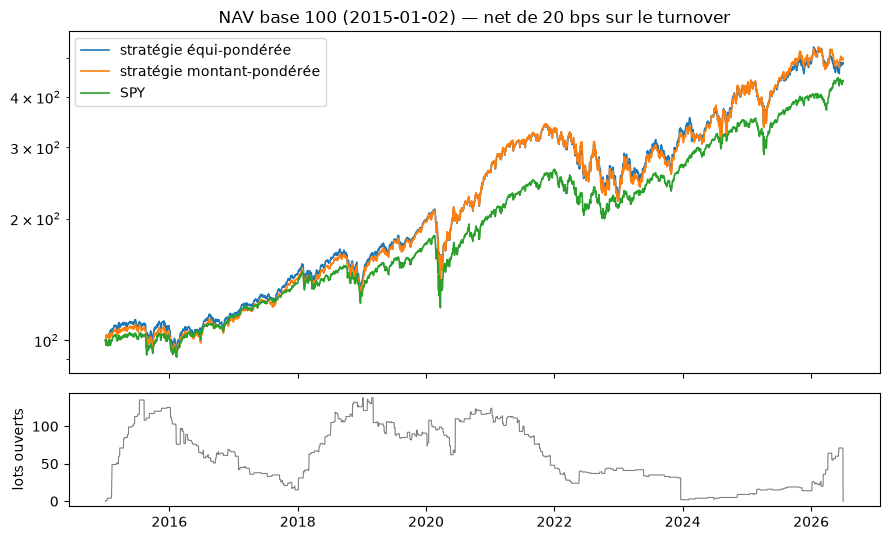
\includegraphics[width=0.92\textwidth]{figures/fig_nav_portefeuille.png}
\caption{NAV base 100 (2015-01-02), nette de 20~bps sur le turnover : stratégie équi-pondérée,
montant-pondérée, et le même argent dans SPY. Bandeau : nombre de lots ouverts.}\label{fig:nav}
\end{figure}

\begin{center}\small
\begin{tabular}{lrrrrrrrr}
\toprule
 & CAGR & vol & Sharpe & maxDD & IR vs SPY & turnover/an & coûts (bps/an) & excès/an \\
\midrule
équi-pondéré & $+14{,}76\,\%$ & $21{,}7\,\%$ & $0{,}74$ & $-35\,\%$ & $0{,}17$ & $7{,}3\times$ & $176$ & $+1{,}95\,\%$ \\
montant-pondéré & $+14{,}98\,\%$ & $22{,}5\,\%$ & $0{,}73$ & $-36\,\%$ & $0{,}19$ & $7{,}4\times$ & $179$ & $+2{,}33\,\%$ \\
équi dédupliqué & $+14{,}54\,\%$ & $21{,}6\,\%$ & $0{,}74$ & $-36\,\%$ & $0{,}16$ & $7{,}2\times$ & $174$ & $+1{,}43\,\%$ \\
\textbf{SPY} & $+13{,}76\,\%$ & $17{,}6\,\%$ & $\mathbf{0{,}82}$ & $-34\,\%$ & --- & --- & --- & --- \\
\bottomrule
\end{tabular}
\end{center}

\subsection{L'année par année --- le test qui compte}
Le juge de paix reste la série des excès annuels, ici \textbf{composés en NAV} :
\begin{equation}
e_Y \;=\; \prod_{t\in Y}\big(1+r_P^{net}(t)\big) \;-\; \prod_{t\in Y}\big(1+r_{SPY}(t)\big)\,,
\qquad t=\frac{\bar e}{s_e/\sqrt{n}}\,,\quad n=12 .
\end{equation}
Différence de convention avec la grille : une année sans nouveau lot n'est plus « 0 » --- le compte y vit
sur ses positions héritées (et un compte vide ferait $e_Y=-r_{SPY,Y}$ : être en cash a un coût
d'opportunité réel).

\begin{figure}[h]\centering
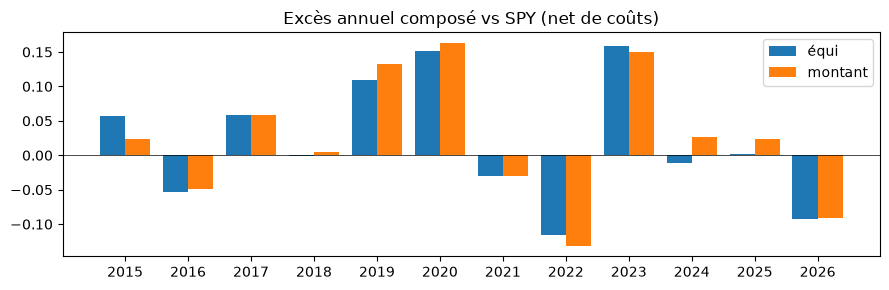
\includegraphics[width=0.92\textwidth]{figures/fig_exces_annuels.png}
\caption{Excès annuel composé vs SPY, net de coûts (équi- et montant-pondéré). Série équi-pondérée : de
$+15{,}9\,\%$ (2023) à $-11{,}5\,\%$ (2022) --- la dispersion écrase la moyenne.}\label{fig:exces}
\end{figure}

\begin{center}\small
\begin{tabular}{lrrrr}
\toprule
 & excès moyen/an & $t$ ($n=12$) & $t$ sans 2026 partielle & années $>0$ \\
\midrule
équi-pondéré & $\mathbf{+1{,}95\,\%}$ & $\mathbf{0{,}76}$ & $1{,}14$ & 50\,\% \\
montant-pondéré & $+2{,}33\,\%$ & $0{,}87$ & $1{,}25$ & 67\,\% \\
\bottomrule
\end{tabular}
\end{center}

\subsection{V2 ETF en compte, et lecture du \S7}
Mêmes lots, mêmes dates, instrument $=$ ETF sectoriel (intersection stricte : 991/1\,037 lots) :

\begin{center}\small
\begin{tabular}{lrrrrrrrr}
\toprule
 & CAGR & vol & Sharpe & maxDD & IR vs SPY & turnover/an & coûts (bps/an) & excès/an \\
\midrule
V1 actions (mêmes lots) & $+14{,}55\,\%$ & $21{,}7\,\%$ & $0{,}73$ & $-35\,\%$ & $0{,}15$ & $7{,}2\times$ & $174$ & $+1{,}76\,\%$ \\
\textbf{V2 ETF sectoriels} & $+13{,}63\,\%$ & $18{,}7\,\%$ & $0{,}78$ & $-35\,\%$ & $\mathbf{0{,}02}$ & $4{,}2\times$ & $100$ & $\mathbf{-0{,}17\,\%}$ \\
\bottomrule
\end{tabular}
\end{center}

\textbf{Lecture --- la vue portefeuille confirme le \S\ref{sec:brief}, et l'affaiblit encore} :
\begin{itemize}[leftmargin=1.4em,itemsep=1pt]
\item Le $+3{,}11\,\%$/trade ne survit pas au passage en compte : excès composé $+1{,}95\,\%$/an (équi,
      $t=0{,}76$) à $+2{,}33\,\%$/an (montant, $t=0{,}87$) --- moins, et encore moins significatif.
\item \textbf{Le client prend plus de risque que SPY pour ça} : Sharpe $0{,}74<0{,}82$, vol $21{,}7$ vs
      $17{,}6\,\%$, même maxDD ($-35\,\%$) ; IR $0{,}17$ : par unité de risque relatif, presque rien.
\item \textbf{Les coûts réels sont lourds} : turnover $\approx7\times$/an $\Rightarrow\approx175$~bps/an de
      drag, dont une bonne part vient du rebalancement quotidien de la discipline équi-pondérée elle-même
      (limite de construction assumée).
\item \textbf{Pas un artefact de sizing} : équi, montant-pondéré et dédupliqué donnent la même image ---
      excès annuel de $+1{,}43$ à $+2{,}33\,\%$/an selon la construction, $t<1$ partout.
\item \textbf{V2 ETF : l'excès disparaît en compte} ($-0{,}17\,\%$/an, IR $0{,}02$) --- la dilution du
      \S\ref{sec:v2}, vue en NAV.
\end{itemize}

% ════════════════════════════════════════════════════════════════════
\section{Verdict}\label{sec:verdict}

\begin{center}\small
\begin{tabular}{p{6.1cm}p{9.3cm}}
\toprule
Question & Réponse (2014--2026, donnée canonique, net de 40~bps A/R) \\
\midrule
De l'info dans les trades, au plafond (\code{transaction\_date}) ? & \textbf{Non} --- achats $-0{,}18\,\%$
(1~m) à $-0{,}76\,\%$ (6~m) vs SPY, $t<-4$. \\
Un drift copiable à la publication ? & Trace réelle ($+7$~bps le 1\textsuperscript{er} mois, $t=1{,}9$)
mais \textbf{6$\times$ sous les coûts}. \\
La stratégie du brief (top-$K$ Sharpe, sortie vente plafonnée 12~m) ? & $+0{,}7$ à $+3{,}6\,\%$/trade selon
config, \textbf{$t\leq1{,}3$ sur les 8 essais} ; le copy-trading non sélectif perd ($-0{,}42\,\%$/trade). \\
Et en compte réel (NAV, coûts sur turnover) ? & Excès composé \textbf{$+1{,}9$ à $+2{,}3\,\%$/an,
$t\leq0{,}9$} ; \textbf{Sharpe $0{,}74<$ SPY $0{,}82$} pour plus de vol ; robuste au sizing. \\
Les 12 leaders de parti (Wei \& Zhou) ? & \textbf{Non testable} : $\sim$6 leaders traders, 89\,\% des
trades $=$ une personne en 2025. \\
La V2 ETF sectorielle ? & Dilution par trade \textbf{et} en compte : excès $\approx0$, IR $0{,}02$ --- le
signal résiduel est spécifique au titre. \\
\bottomrule
\end{tabular}
\end{center}

\textbf{Ce que ça veut dire pour Ramify} :
\begin{itemize}[leftmargin=1.4em,itemsep=1pt]
\item Notre résultat \textbf{réplique le consensus} académique (Belmont~2022 : pas d'alpha moyen
      post-STOCK Act) et le marché réel (NANC : $+2{,}7$~pt/an vs SPY depuis 2023 mais $-3{,}8$~pt vs QQQ
      --- du style, pas du talent). Ce qui reste est une loterie à queue droite qu'une sélection ex-ante
      ne capte pas.
\item Un produit « Congrès » se défend comme \textbf{bêta thématique transparent}, pas comme une promesse
      de battre le marché.
\item \textbf{Pistes non testées ici} (cf. \code{ETAT\_DE\_L\_ART\_STRATEGIES.md}) : juridiction de comité
      $\times$ industrie ($+50$~bps à l'annonce), trades $\times$ jalons législatifs (Li~2025 :
      $+3$--$5\,\%$), conviction par taille (« Best Ideas »). Matière pour une v2.
\item \textbf{Risque réglementaire} : le HONEST Act (interdiction du trading des élus) a passé la
      commission sénatoriale en 2025 --- toute mise en production vivrait sous ce risque d'extinction.
\end{itemize}

\textbf{Limites assumées} : $t$ simples (fenêtres chevauchantes et lots multi-comptes $\Rightarrow$ $t$
optimistes --- ils ne sont déjà pas significatifs) ; couverture prix $87{,}8\,\%$, plus trouée en début de
fenêtre ($\sim74\,\%$ en 2014) $\Rightarrow$ léger biais de survie ; construction en poids rebalancée
quotidiennement (le drag $\approx175$~bps/an inclut le rebalancement de la discipline équi-pondérée) ;
cash à 0\,\% ; pas de slippage au-delà des 20~bps ; prix \emph{ffillés} (dernier cours connu) pour les
délistés en cours de détention ; 10\,\% des achats récents ont une détention tronquée au 2026-07-02.

% ════════════════════════════════════════════════════════════════════
\appendix
\section{Traçabilité rapport $\leftrightarrow$ notebook}\label{app:trace}
Chaque chiffre de ce rapport est la sortie d'une cellule de
\code{06\_Recherche\_Strategie\_2014\_2026.ipynb} (42~cellules ; numérotation 0-based du JSON, la
cellule~0 étant le titre) :
\begin{center}\small
\begin{tabular}{ll}
\toprule
Section du rapport & Cellules du notebook \\
\midrule
\S\ref{sec:donnees} données, cache prix, panel & 1--5 (cellule 4 $=$ construction du cache) \\
\S\ref{sec:mesure} mesure de base, exemple Pelosi/NVDA & 6--8 \\
\S\ref{sec:evenement} événement (2 dates $\times$ 5 horizons) & 9--12 \\
\S\ref{sec:brief} appariement, track record, grille & 13--21 \\
\S\ref{sec:variantes} leaders, horizon court & 22--25 \\
\S\ref{sec:v2} V2 ETF par trade & 26--27 \\
\S\ref{sec:ptf} portefeuille (moteur, contrôles, stats, V2) & 28--40 \\
\S\ref{sec:verdict} verdict & 41 \\
\bottomrule
\end{tabular}
\end{center}

\section{Reproductibilité}
Le notebook est \textbf{auto-suffisant} : ouvert sur le kernel du dépôt (\code{.venv}) et exécuté de haut
en bas, il (re)construit au besoin son cache de prix (cellule 4 --- resumable, $0$~appel réseau si le
cache est complet), puis produit chaque chiffre et les deux figures de ce rapport (extraites telles
quelles des sorties). Entrées en lecture seule : la table canonique
\code{00\_S1S2\_donnees/data/clean/transactions\_backtest\_2014\_2026.csv} (134\,464 lignes, certifiée par
\code{docs/RAPPORT\_QUALITE.md}) et \code{leadership\_2014\_2026.csv} (50~mandats vérifiés). Dépendances :
\code{numpy}, \code{pandas}, \code{matplotlib} (+\code{yfinance} uniquement si le cache est incomplet).
Aucun aléa : deux exécutions donnent les mêmes sorties octet pour octet.

\end{document}
